\section{Langkah-Langkah Percobaan}
\subsection{Crimping}
\begin{enumerate}
    \item Siapkan alat: kabel UTP, konektor RJ-45, crimping tool.
    \item Kupas jaket kabel ±2-3 cm.
    \item Pisahkan dan luruskan 8 kabel kecil.
    \item Susun kabel sesuai urutan warna.
    \item Potong ujung kabel agar rata.
    \item Masukkan kabel ke konektor RJ-45.
    \item Crimping dengan crimping tool.
    \item Ulangi di ujung kabel satunya.
    \item Tes dengan kabel tester.
\end{enumerate}

\subsection{Static Routing}
\begin{enumerate}
    \item Sambungkan kabel LAN ke laptop dan buka aplikasi WinBox.
    \item Buka menu Neighbours di WinBox, pilih MAC address router yang terdeteksi, lalu klik Connect.
    \item Di menu utama, masuk ke System > Reset Configuration, centang opsi No Default Configuration, lalu klik Reset Configuration.
    \item Tunggu hingga router selesai restart, kemudian sambungkan kembali ke WinBox
    \item Hubungkan Router 1 ke Router 2 melalui kabel LAN di port ether7, dan sambungkan ether6 ke laptop.
    \item Di WinBox, buka IP > Address List, klik tombol +, lalu masukkan alamat IP router ( 10.10.10.1/30 untuk jaringan antar-router 10.10.10.0 dan pilih interface ether7.
    \item Tambahkan lagi alamat IP untuk laptop di jaringan yang berbeda dan pilih interface yang sesuai.
    \begin{figure}[H]
        \centering
        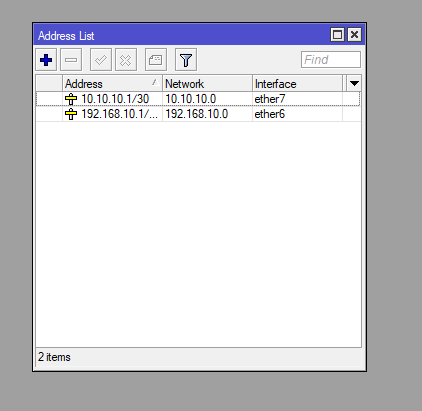
\includegraphics[width=0.5\linewidth]{address list static.png}
        \caption{Address Router 1}
        \label{fig:enter-label}
    \end{figure}
    \item Ulangi tahap yang sama ke router 2
    \begin{figure}[H]
        \centering
        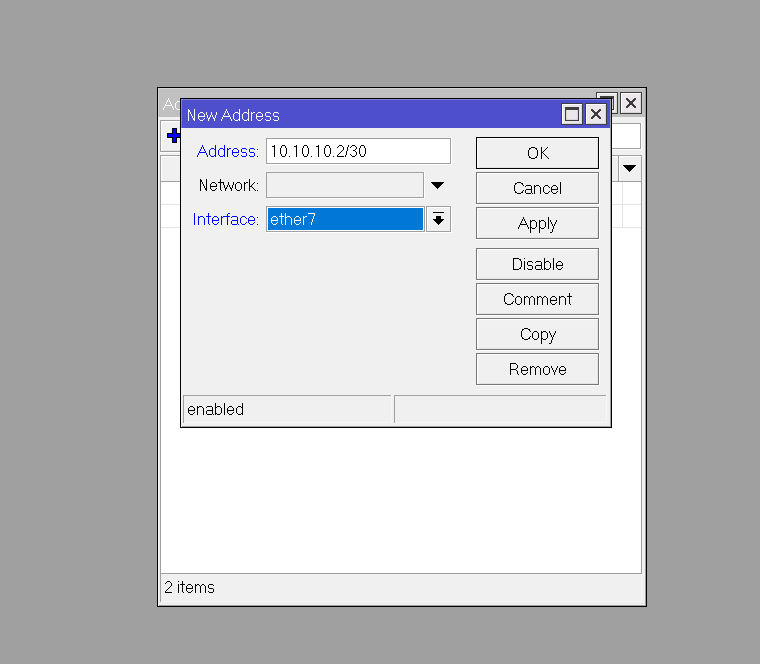
\includegraphics[width=0.5\linewidth]{address router 2.png}
        \caption{Address Router 2}
        \label{fig:enter-label}
    \end{figure}
    \begin{figure}[H]
        \centering
        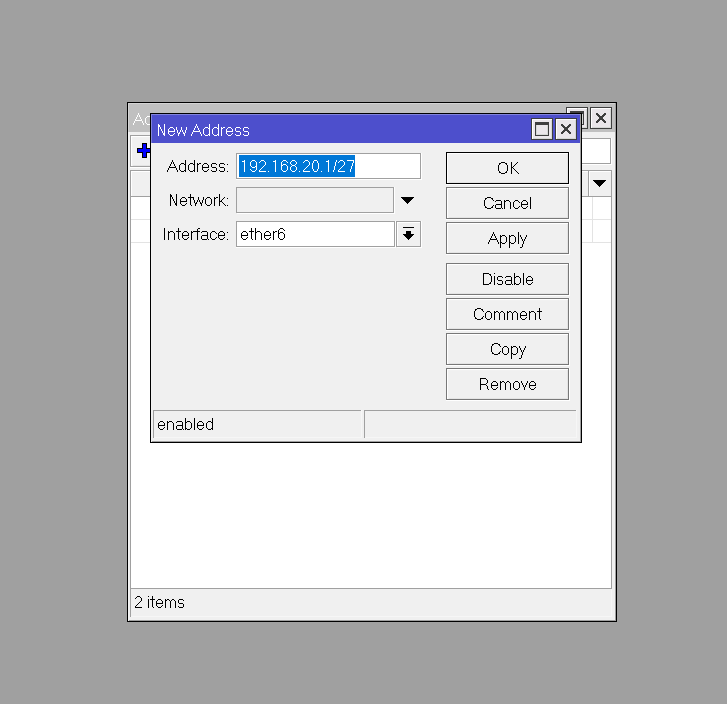
\includegraphics[width=0.5\linewidth]{address laptop 2.png}
        \caption{Address Laptop 2}
        \label{fig:enter-label}
    \end{figure}
    \item Di WinBox, buka menu IP > Routes.
    \item Klik tombol + untuk menambahkan route. Isi Address dengan alamat network tujuan Router 1: 192.168.20.0/27, Router 2: 192.168.10.0/27 dan Gateway dengan alamat router tujuan Router 1: 10.10.10.2, Router 2: 10.10.10.1.
    \begin{figure}[H]
        \centering
        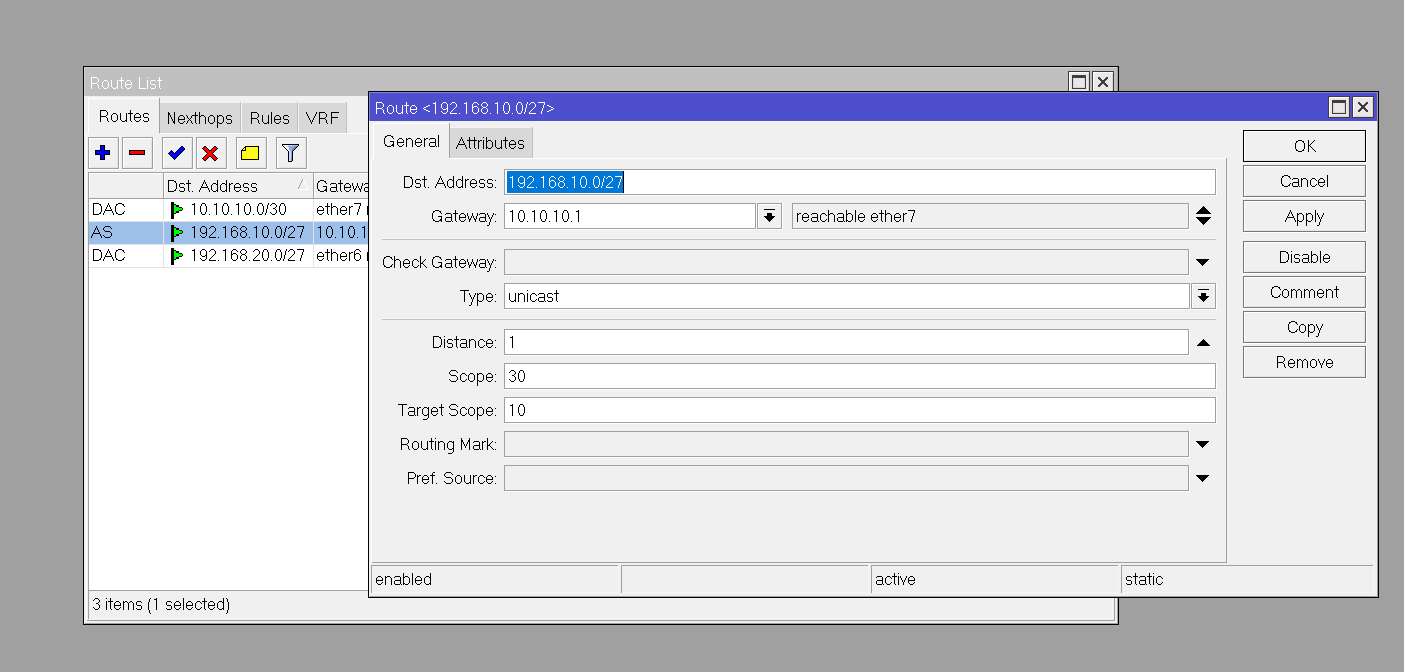
\includegraphics[width=0.5\linewidth]{Screenshot 2025-05-10 161521.png}
        \caption{Router List 2}
        \label{fig:enter-label}
    \end{figure}
    \begin{figure}[H]
        \centering
        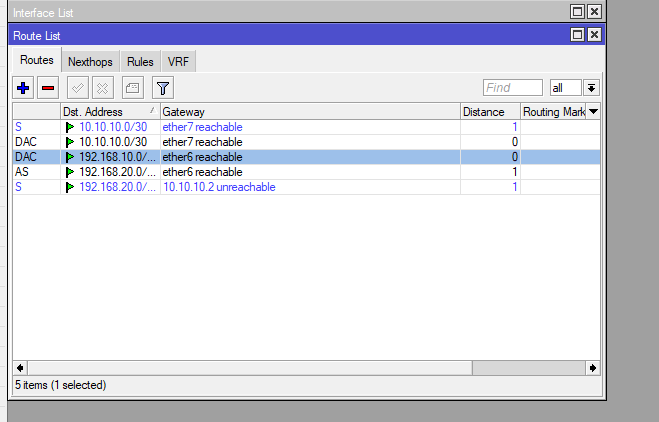
\includegraphics[width=0.5\linewidth]{route list statis.png}
        \caption{Route List 1}
        \label{fig:enter-label}
    \end{figure}
    \item Masuk ke pengaturan jaringan di laptop, ubah IP menjadi manual, lalu masukkan IP Address sesuai kebutuhan, netmask /27 (255.255.255.224), dan gateway sesuai jaringan yang digunakan. Lakukan pengaturan ini pada kedua laptop.
    \item Lakukan uji koneksi dengan perintah ping ke kedua router dan laptop di jaringan berbeda melalui terminal di masing-masing laptop.
    \begin{figure}[H]
        \centering
        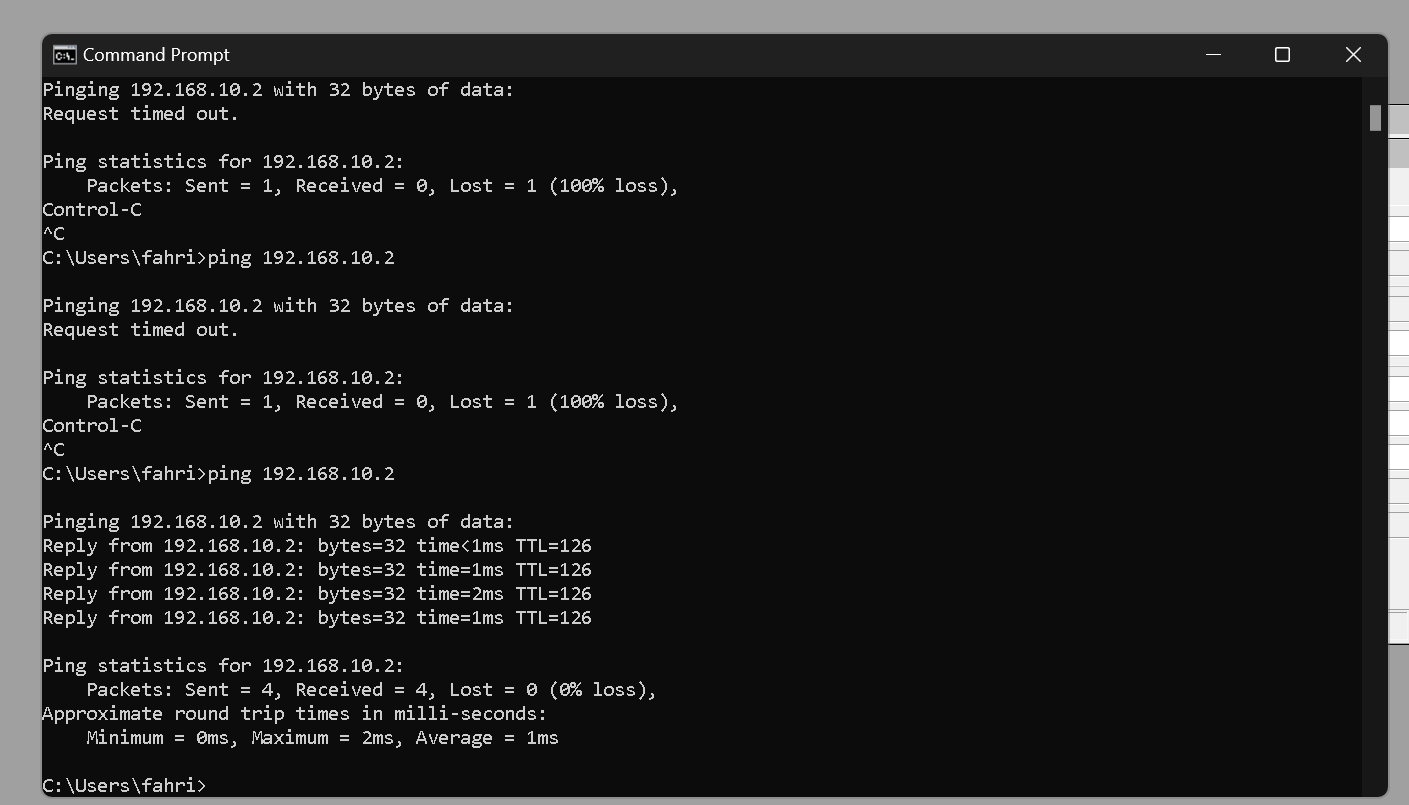
\includegraphics[width=0.5\linewidth]{ping laptop 2 ke laptop 1.png}
        \caption{Ping Laptop 2 ke 1}
        \label{fig:enter-label}
    \end{figure}
    \begin{figure}[H]
        \centering
        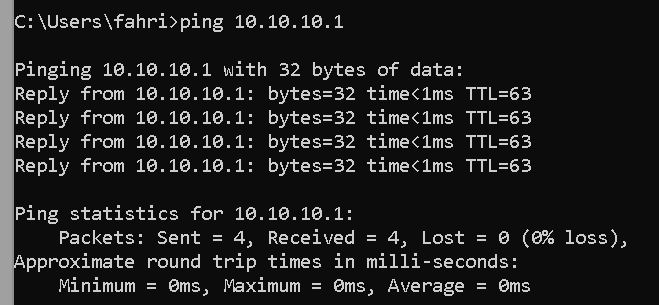
\includegraphics[width=0.5\linewidth]{ping laptop 2 ke router 1.png}
        \caption{Ping Laptop 2 ke Router 1}
        \label{fig:enter-label}
    \end{figure}
    \begin{figure}[H]
        \centering
        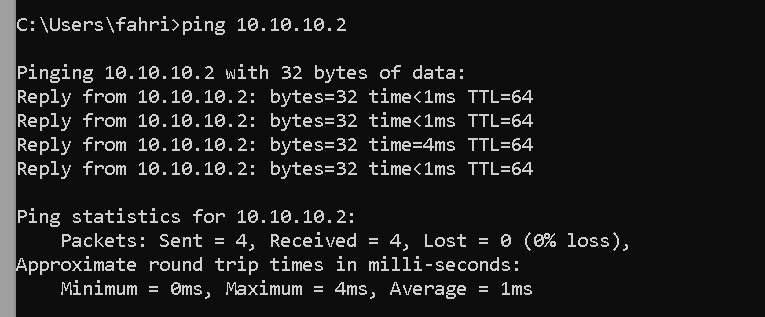
\includegraphics[width=0.5\linewidth]{ping laptop 2 ke royter 2.png}
        \caption{Ping Laptop 2 Ke Router 2}
        \label{fig:enter-label}
    \end{figure}
    \begin{figure}[H]
        \centering
        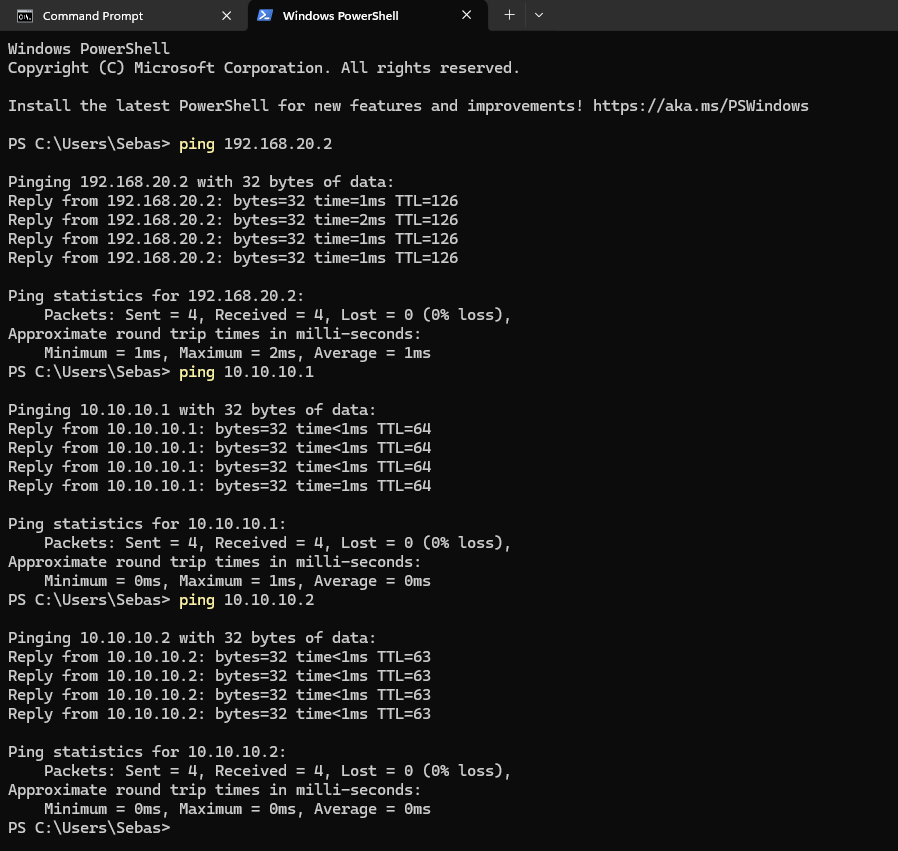
\includegraphics[width=0.5\linewidth]{static.png}
        \caption{Ping Laptop 1 Ke Laptop 2, Router 1, dan router 2}
        \label{fig:enter-label}
    \end{figure}
\end{enumerate}

\subsection{Dynamic Routing}
\begin{enumerate}
    \item Di WinBox, hapus daftar static route dengan memilih route yang ada lalu klik tombol (-).
    \item Buka menu IP > DHCP Server, lalu klik DHCP Setup dan pilih interface ether6.
    \item Masuk ke menu Routing > RIP, tambahkan interface dan pilih ether all, set Receive ke V1-V2, Send ke V2, dan biarkan Authentication sebagai none.
    \begin{figure}[H]
        \centering
        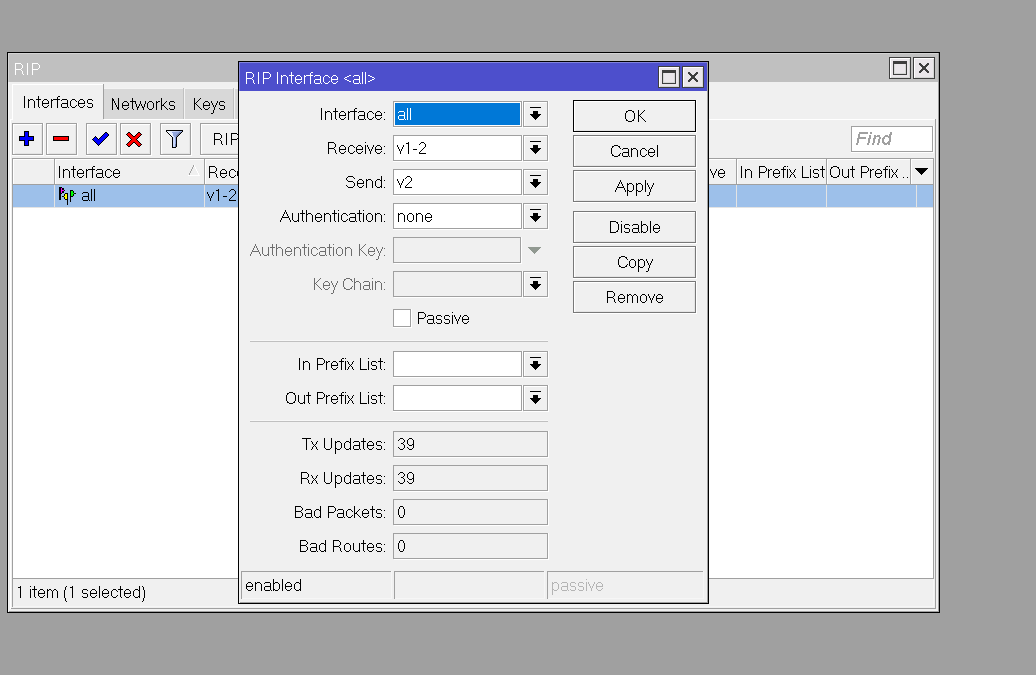
\includegraphics[width=0.5\linewidth]{RIP Router 2.png}
        \caption{RIP Router 2}
        \label{fig:enter-label}
    \end{figure}
    \begin{figure}[H]
        \centering
        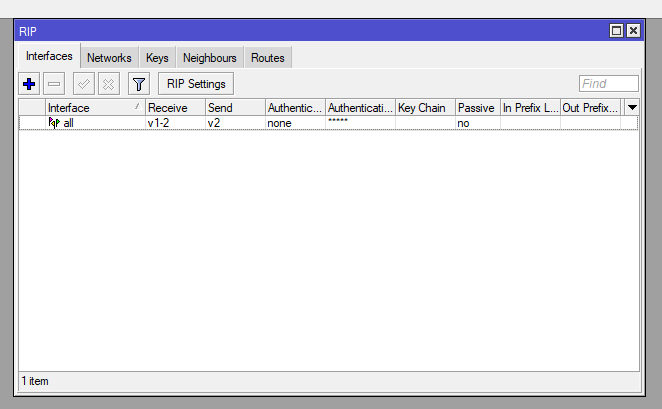
\includegraphics[width=0.5\linewidth]{rip interfaces.png}
        \caption{RIP Router 1}
        \label{fig:enter-label}
    \end{figure}
    \item Di menu RIP, buka tab Networks, lalu masukkan semua alamat IP network yang terhubung ke router.
    \begin{figure}[H]
        \centering
        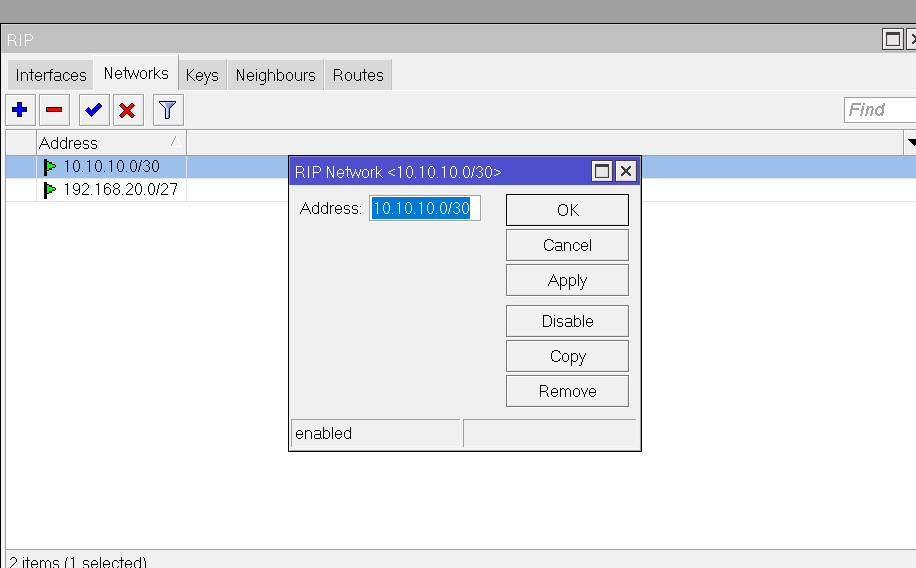
\includegraphics[width=0.5\linewidth]{rip netwoerk router 2.png}
        \caption{RIP Network 2}
        \label{fig:enter-label}
    \end{figure}
    \begin{figure}[H]
        \centering
        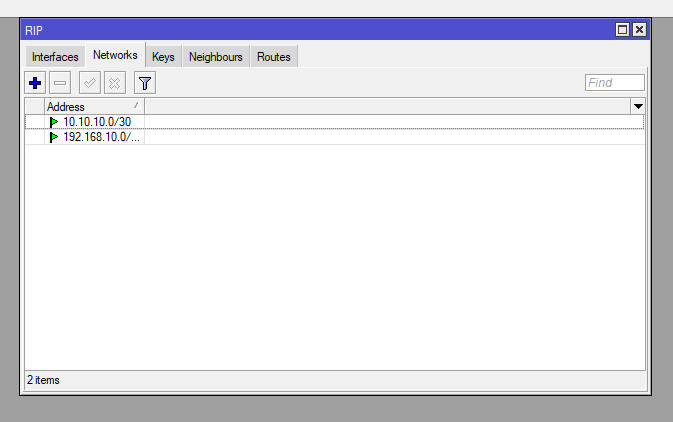
\includegraphics[width=0.5\linewidth]{rip networks.png}
        \caption{RIP Network 1}
        \label{fig:enter-label}
    \end{figure}
    \item Buka tab Neighbours pada menu RIP, lalu masukkan gateway dari laptop tujuan (destinasi).
    \begin{figure}[H]
        \centering
        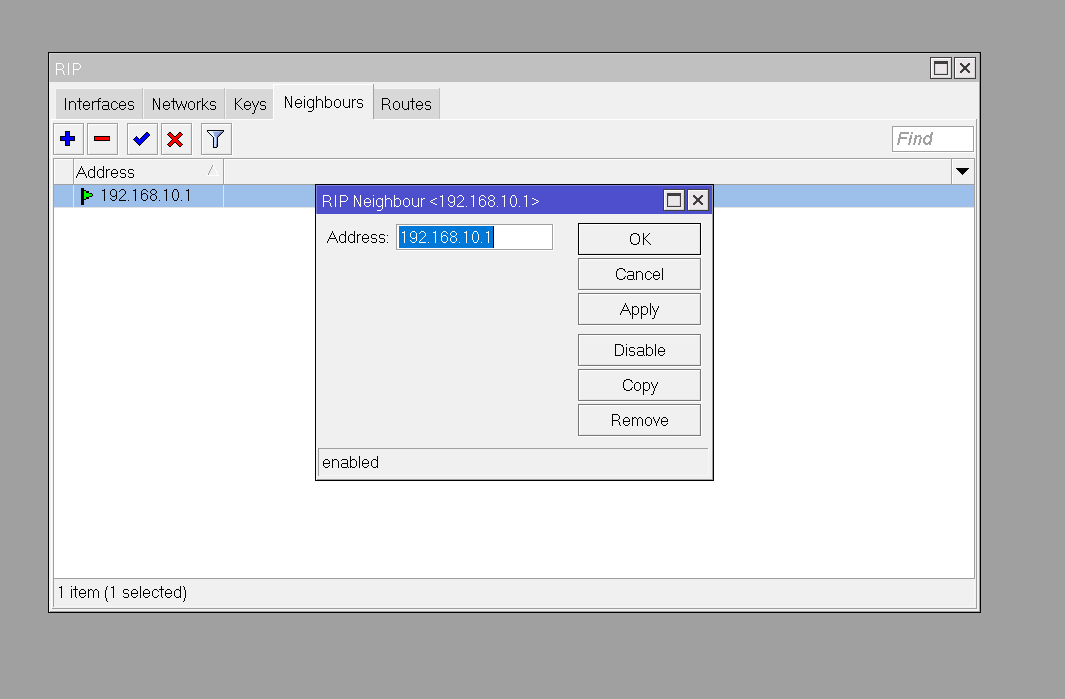
\includegraphics[width=0.5\linewidth]{RIP Neighbour Router 2.png}
        \caption{RIP Neighbour 2}
        \label{fig:enter-label}
    \end{figure}
    \begin{figure}[H]
        \centering
        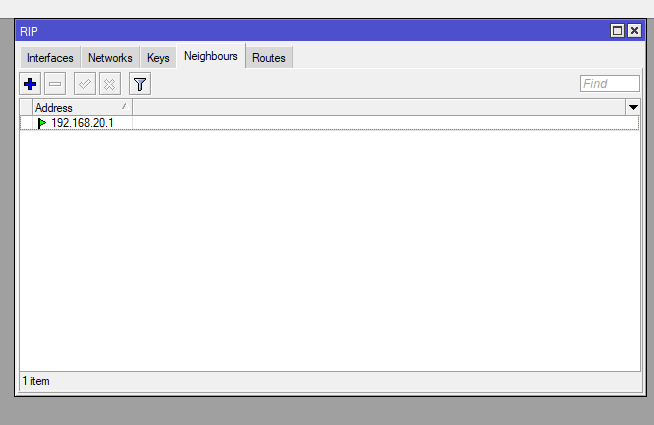
\includegraphics[width=0.5\linewidth]{rip neighbours.png}
        \caption{RIP Neighbour 1}
        \label{fig:enter-label}
    \end{figure}
    \item Lalu ubah pengaturan IP menjadi DHCP, lalu lakukan ping test ke antar laptop, Router 1, dan Router 2 untuk memastikan koneksi berhasil.
\end{enumerate}

\section{Analisis Hasil Percobaan}
Pada Percobaan 1 dilakukan proses crimping kabel UTP, yang terdiri dari delapan inti kabel di dalamnya. Masing-masing kabel memiliki fungsi berbeda, seperti untuk transmisi data (TX – oranye), penerimaan data (RX – hijau), dan daya (cokelat). Beberapa kabel memiliki strip putih yang menunjukkan pasangan positif dari warna tersebut. Kabel UTP memiliki beberapa kategori, dan dalam praktikum ini digunakan kabel UTP kategori CAT5, yang tidak dilengkapi fitur grounding. Oleh karena itu, ketika diuji menggunakan LAN Tester, indikator LED untuk kabel grounding tidak menyala. Percobaan 2 berfokus pada konfigurasi routing statis menggunakan dua router dan dua laptop. Topologi jaringan terdiri dari tiga segmen: network 10.10.10.0/30 digunakan sebagai jaringan antar-router, network 192.168.10.0/27 menghubungkan Router 1 dengan Laptop 1, dan network 192.168.20.0/27 menghubungkan Router 2 dengan Laptop 2. CIDR /30 membatasi jaringan antar-router hanya memiliki dua IP yang bisa digunakan, sementara CIDR /27 memungkinkan hingga 30 alamat IP untuk perangkat pengguna. Konfigurasi IP dilakukan melalui menu Address List pada router, dengan memilih interface yang sesuai. Misalnya, interface ether7 yang menghubungkan antar-router diberi alamat 10.10.10.1/30. Untuk menentukan arah lalu lintas data, digunakan pengaturan pada Route List dengan menambahkan destination address dan gateway yang dituju. Selama pengujian, ping antar laptop gagal karena firewall di laptop penerima memblokir paket yang masuk. Pada Percobaan 3 dilakukan konfigurasi routing dinamis. Routing dinamis memungkinkan perangkat dalam jaringan untuk secara otomatis mendapatkan IP address dan membentuk topologi jaringan menggunakan protokol tertentu, yaitu Routing Information Protocol (RIP). Pengaturan RIP dilakukan dengan menentukan interface yang digunakan, menambahkan network yang terhubung, dan gateway yang berpartisipasi dalam pertukaran informasi routing. RIP secara otomatis menyebarkan informasi rute ke perangkat lain, sehingga konfigurasi jaringan menjadi lebih efisien tanpa perlu penambahan rute secara manual.


\section{Hasil Tugas Modul}
\begin{enumerate}
    \item Topologi Di Cisco
    \begin{figure}[H]
        \centering
        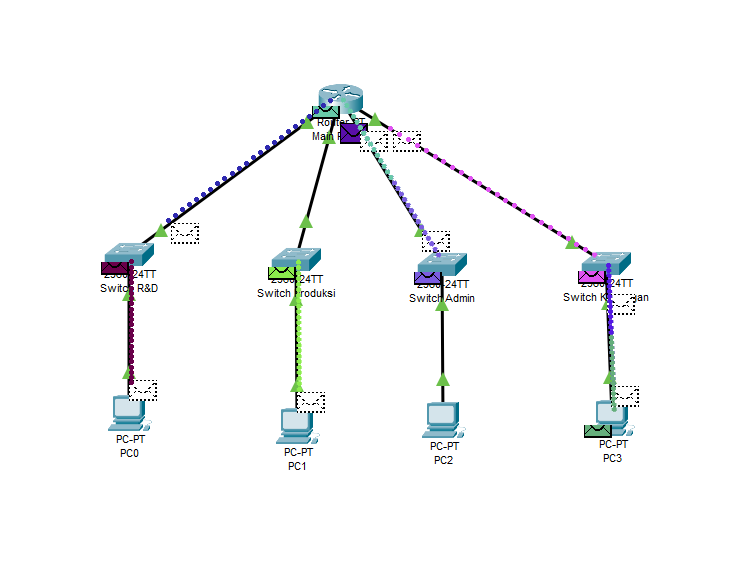
\includegraphics[width=0.5\linewidth]{cisco.png}
    \end{figure}
    \item mengalami kesulitan dalam menggunakan Winbox karena masih banyak hal yang belum saya pahami 
\end{enumerate}

\section{Kesimpulan}
Pada Static Routing, pengaturan IP dan routing dilakukan secara manual. Setiap perangkat harus dikonfigurasi dengan alamat IP yang sesuai dan dihubungkan antar-network melalui pengaturan routing berdasarkan interface yang digunakan. Hal ini memerlukan pemahaman topologi jaringan dan konfigurasi yang teliti. Sementara itu, pada Dynamic Routing, proses konfigurasi dilakukan secara otomatis. Perangkat hanya perlu diatur dengan protokol routing yang digunakan, seperti RIP, sehingga IP dan informasi rute antar-perangkat dapat dibagikan secara otomatis tanpa konfigurasi manual di setiap titik.
\section{Lampiran}
\subsection{Hasil Challenge Modul}
Dibawah berikut merupakan dokumentasi hasil challenge :
\begin{figure}[H]
    \centering
    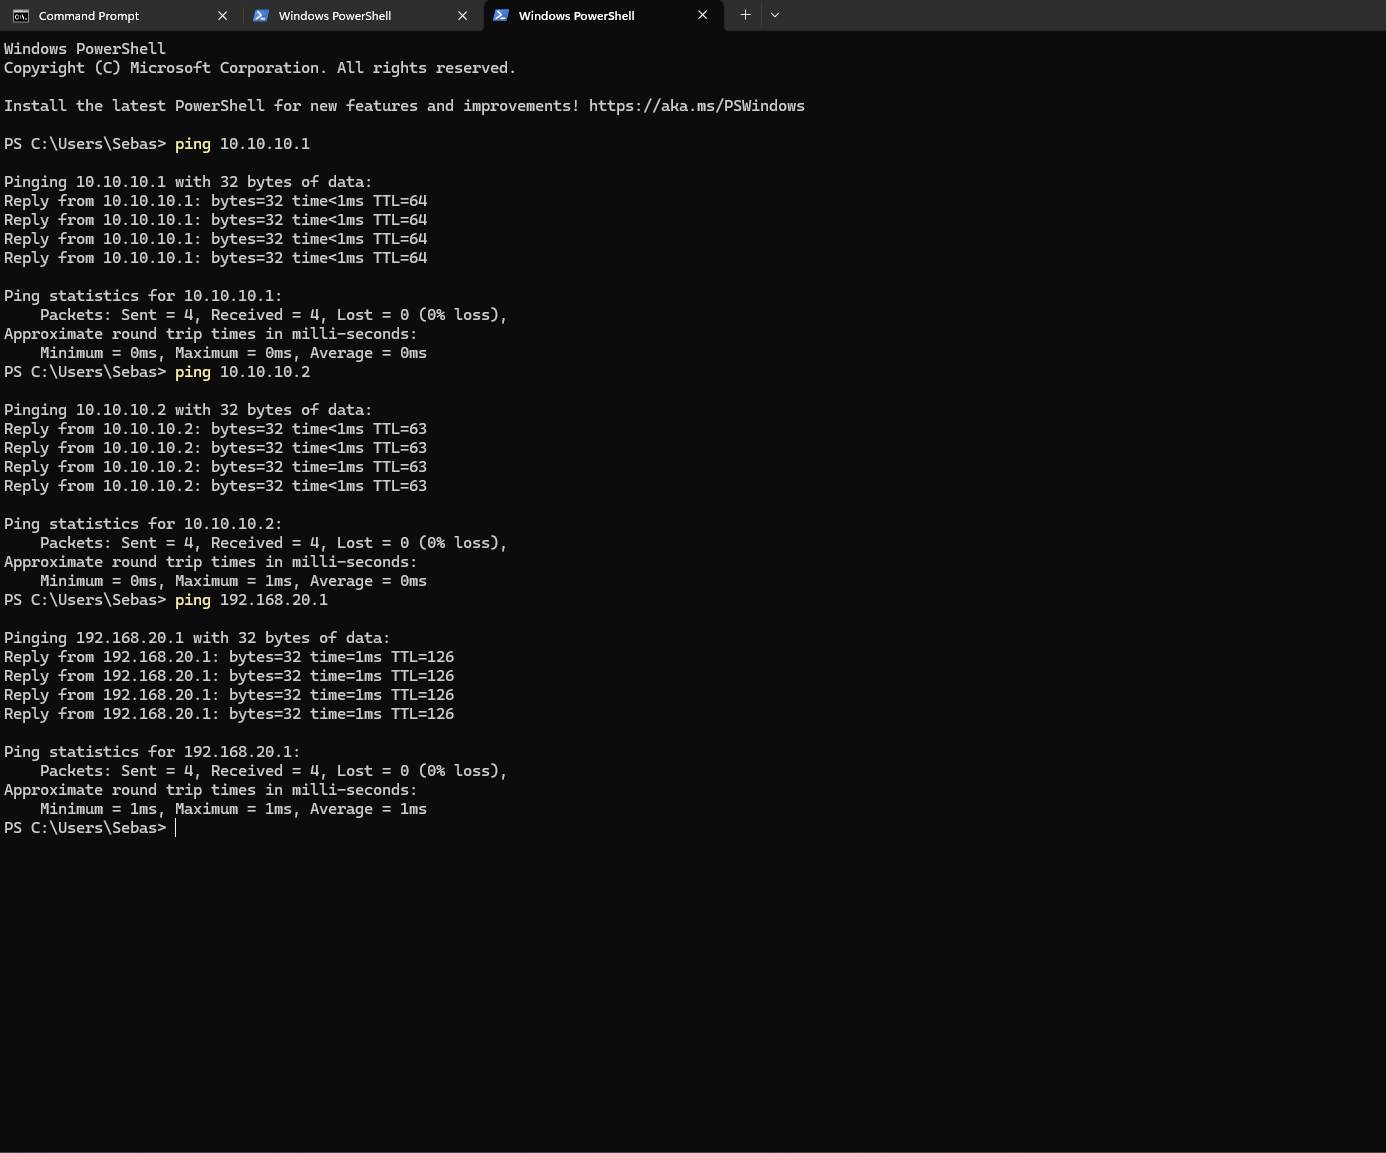
\includegraphics[width=0.5\linewidth]{Screenshot 2025-05-10 164954.png}
\end{figure}
